\documentclass[12pt]{article}

\usepackage{amsmath,amsthm,amsfonts,amssymb,amsxtra}
\usepackage{pgf,tikz}
\usetikzlibrary{arrows}
\renewcommand{\theenumi}{(\alph{enumi})} 
\renewcommand{\labelenumi}{\theenumi}

\pagestyle{empty}
\setlength{\textwidth}{7in}
\setlength{\oddsidemargin}{-0.5in}
\setlength{\topmargin}{-1.0in}
\setlength{\textheight}{9.5in}

\theoremstyle{definition}
\newtheorem{problem}{Problem}

\begin{document}

\noindent{\large\bf MATH 241}\hfill{\large\bf Final Exam.}\hfill{\large\bf
  Spring 2017}\hfill{\large\bf Page 1/8}\hrule

\bigskip
\begin{center}
  \begin{tabular}{|ll|}
    \hline & \cr
    {\bf Name: } & \makebox[12cm]{\hrulefill}\cr & \cr
    {\bf VIP ID:} & \makebox[12cm]{\hrulefill}\cr & \cr
    \hline
  \end{tabular}
\end{center}
\begin{itemize}
\item Write your name and your VIP ID in the space provided above.
\item The test has nine (9) pages, including this one, and the formula sheet attached at the end. 
\item You have 150 minutes to complete this test.
\item Each problem is worth 10 points.
\item Enter your answer in the box(es) provided.
\item You must show sufficient work to justify all answers unless otherwise stated in the problem.  Correct answers with inconsistent work may not be given credit.
\item No books, notes or calculators may be used on this test.
\end{itemize}
\hrule

 \begin{center}
   \begin{tabular}{|c|c|c|}
     \hline
     &&\cr
     {\large\bf Page} & {\large\bf Max} & {\large\bf Points} \cr
     &&\cr
     \hline
     &&\cr
     {\Large 2} & \Large 10 & \cr
     &&\cr
     \hline
     &&\cr
     {\Large 3} & \Large 20 & \cr
     &&\cr
     \hline
     &&\cr
     {\Large 4} & \Large 20 & \cr
     &&\cr
     \hline
     &&\cr
     {\Large 5} & \Large 20 & \cr
     &&\cr
     \hline
     &&\cr
     {\Large 6} & \Large 10 & \cr
     &&\cr
     \hline
     &&\cr
     {\Large 7} & \Large 10 & \cr
     &&\cr
     \hline
     &&\cr
     {\Large 8} & \Large 10 & \cr
     &&\cr
     \hline\hline
     &&\cr
     {\large\bf Total} & \Large 100 & \cr
     &&\cr
     \hline
   \end{tabular}
   \end{center}
\newpage

%%%%%%%%%%%%%%%%%%%%%%%%%%%%%%%%%%%%% Page 2
\noindent{\large\bf MATH 241}\hfill{\large\bf Final Exam.}\hfill{\large\bf
  Spring 2017}\hfill{\large\bf Page 2/8}\hrule

\bigskip
\begin{problem}
Let $\boldsymbol{u} = 6\boldsymbol{i}-\boldsymbol{j}+\boldsymbol{k}$, $\boldsymbol{v}=-12\boldsymbol{i}+2\boldsymbol{j}-2\boldsymbol{k}$, $\boldsymbol{w} = \boldsymbol{j}-6\boldsymbol{k}$.  
\begin{enumerate}
\item (4 pts) Which of those vectors are perpendicular? 
\vspace{4cm}
\begin{flushright}
  \begin{tikzpicture}
    \draw (0cm,-0.2cm) rectangle (5cm,1.2cm);
  \end{tikzpicture}
\end{flushright}
\item (4 pts) Which of those vectors are parallel?
\vspace{4cm}
\begin{flushright}
  \begin{tikzpicture}
    \draw (0cm,-0.2cm) rectangle (5cm,1.2cm);
  \end{tikzpicture}
\end{flushright}
\item (2 pts) What is the volume of the parallelepiped determined by $\boldsymbol{u}, \boldsymbol{v}$ and $\boldsymbol{w}$?
\vspace{5cm}
\begin{flushright}
  \begin{tikzpicture}
    \draw (-0.5cm,0.5cm) node {$V = $};
    \draw (0cm,-0.2cm) rectangle (5cm,1.2cm);
  \end{tikzpicture}
\end{flushright}
\end{enumerate}
\end{problem}
\newpage

%%%%%%%%%%%%%%%%%%%%%%%%%%%%%%%%%%%%% Page 3
\noindent{\large\bf MATH 241}\hfill{\large\bf Final Exam.}\hfill{\large\bf
  Spring 2017}\hfill{\large\bf Page 3/8}\hrule

\bigskip
\begin{problem}[10 pts]
Find an equation of the plane determined by the intersecting lines
\begin{equation*}
L_1: \begin{cases}
x &= -1+t \\
y &= 2+3t \\
z &= 1-4t
\end{cases} \qquad
L_2: \begin{cases}
x &= 1 - 4s \\
y &= 1 + 2s \\
z &= 2 - 2s
\end{cases}
\end{equation*}
\vspace{8.5cm}
\begin{flushright}
  \begin{tikzpicture}
    \draw (-0.75cm,0.5cm) node {plane:};
    \draw (0cm,-0.2cm) rectangle (10cm,1.2cm);
  \end{tikzpicture}
\end{flushright}
\end{problem}
\hrule
\begin{problem}[10 pts]
Find the distance from the point $(0,6,0)$ to the plane $4x+7y+4z=32$.
\vspace{7.75cm}
\begin{flushright}
  \begin{tikzpicture}
    \draw (-1cm,0.5cm) node {$d =$};
    \draw (0cm,-0.2cm) rectangle (5cm,1.2cm);
  \end{tikzpicture}
\end{flushright}
\end{problem}
\newpage

%%%%%%%%%%%%%%%%%%%%%%%%%%%%%%%%%%%%% Page 4
\noindent{\large\bf MATH 241}\hfill{\large\bf Final Exam.}\hfill{\large\bf
  Spring 2017}\hfill{\large\bf Page 4/8}\hrule

\bigskip
\begin{problem}[10 pts]
Find the following limit, or prove that it does not exist:
\begin{equation*}
\lim_{(x,y)\to(0,0)} \frac{2x}{x^2+x+y^2}
\end{equation*}
\vspace{8.5cm}
\begin{flushright}
  \begin{tikzpicture}
    \draw (-2.5cm,0.5cm) node {$\displaystyle{\lim_{(x,y)\to(0,0)} \dfrac{2x}{x^2+x+y^2} =}$};
    \draw (0cm,-0.2cm) rectangle (5cm,1.2cm);
  \end{tikzpicture}
\end{flushright}
\end{problem}
\hrule
\begin{problem}[10 pts]
Find the line integral of $f(x,y,z)=x+y+z$ over the straight-line segment from $(2,3,1)$ to $(1,-1,-1)$.
\vspace{8cm}
\begin{flushright}
  \begin{tikzpicture}
    \draw (-1cm,0.5cm) node {$\int_C f\, ds =$};
    \draw (0cm,-0.2cm) rectangle (5cm,1.2cm);
  \end{tikzpicture}
\end{flushright}
\end{problem}
\newpage

%%%%%%%%%%%%%%%%%%%%%%%%%%%%%%%%%%%%% Page 5
\noindent{\large\bf MATH 241}\hfill{\large\bf Final Exam.}\hfill{\large\bf
  Spring 2017}\hfill{\large\bf Page 5/8}\hrule

\bigskip
\begin{problem}[10 pts]
Find the curvature $\kappa(t)$ of the vector function $\boldsymbol{r}(t) = \frac{t^5}{5}\boldsymbol{i} + \frac{t^2}{2}\boldsymbol{j}$, $t>0$.
\vspace{5cm}
\begin{flushright}
  \begin{tikzpicture}
    \draw (13cm,2.5cm) node {$\kappa(t) = $};
    \draw (13.75cm,1.7cm) rectangle (23cm,3.2cm);
  \end{tikzpicture}
\end{flushright}
\end{problem}
\hrule
\begin{problem}[10 pts]
Find all the local maxima, local minima, and saddle points of the function $fx,y) = x^3+y^3+3x^2-9y^2-1$.
\end{problem}

\newpage

%%%%%%%%%%%%%%%%%%%%%%%%%%%%%%%%%%%%% Page 6
\noindent{\large\bf MATH 241}\hfill{\large\bf Final Exam.}\hfill{\large\bf
  Spring 2017}\hfill{\large\bf Page 6/8}\hrule

\bigskip
\begin{problem}[10 pts]
Find the absolute maximum and minimum (both location and value) of the function $f(x,y) = 7x^2+8y^2$ on the closed triangular region bounded by the lines $x=0$, $y=0$, $y+2x=2$ in the first quadrant.  Sketch the region.

\vspace{0.5cm}
\begin{tikzpicture}[scale=0.7]
  \draw [white] (-0.5,-0.5) rectangle (6.5,6.5);
  \draw [<->, ultra thick] (-0.5,0) -- (6.5,0);
  \draw [<->, ultra thick] (0,-0.5) -- (0,6.5);
  \draw[step=0.5,gray,ultra thin] (-0.25, -0.25) grid (6.25, 6.25);
  \end{tikzpicture}
\vspace{14cm}
\begin{flushright}
  \begin{tikzpicture}
    \draw (0cm,0.5cm) node {Maximum:};
    \draw (1.2cm,-0.2cm) rectangle (7.2cm,1.2cm);
    \draw (9cm,0.5cm) node {Minimum:};
    \draw (10.2cm,-0.2cm) rectangle (16.2cm,1.2cm);
  \end{tikzpicture}
\end{flushright}
\end{problem}
\newpage

%%%%%%%%%%%%%%%%%%%%%%%%%%%%%%%%%%%%% Page 7
\noindent{\large\bf MATH 241}\hfill{\large\bf Final Exam.}\hfill{\large\bf
  Spring 2017}\hfill{\large\bf Page 7/8}\hrule

\bigskip
\begin{problem}[10 pts]
Given the integral below:  Sketch the domain of integration, change the integral into an equivalent polar integral, and evaluate the polar integral.
\begin{equation*}
\int_{-1}^0 \int_{-\sqrt{1-x^2}}^0 \, \frac{6}{1+\sqrt{x^2+y^2}}\, dy\, dx
\end{equation*}
\vspace{0.5cm}
\begin{tikzpicture}[scale=0.7]
  \draw [white] (-0.5,-0.5) rectangle (6.5,6.5);
  \draw [<->, ultra thick] (-0.5,3) -- (6.5,3);
  \draw [<->, ultra thick] (3,-0.5) -- (3,6.5);
  \draw[step=0.5,gray,ultra thin] (-0.25, -0.25) grid (6.25, 6.25);
  \end{tikzpicture}
\vspace{12cm}
\begin{flushright}
  \begin{tikzpicture}
    \draw (0cm,0.5cm) node {$\displaystyle{\int_{-1}^0 \int_{-\sqrt{1-x^2}}^0 \, \frac{6}{1+\sqrt{x^2+y^2}}\, dy\, dx}=$};
    \draw (3.5cm,-0.3cm) rectangle (11.5cm,1.3cm);
    \draw (12cm,0.5cm) node {$=$};
    \draw (12.5cm,-0.3cm) rectangle (15cm,1.3cm);
  \end{tikzpicture}
\end{flushright}
\end{problem}
\newpage

%%%%%%%%%%%%%%%%%%%%%%%%%%%%%%%%%%%%% Page 8
\noindent{\large\bf MATH 241}\hfill{\large\bf Final Exam.}\hfill{\large\bf
  Spring 2017}\hfill{\large\bf Page 8/8}\hrule

\bigskip
\begin{problem}[10 pts]
We want to find the volume of the solid cut from the thick-walled cylinder $1\leq x^2+y^2 \leq 6$ by the cones $z = \pm \sqrt{4x^2+4y^2}$.  Sketch that solid, find an integral expression that computes its volume (double or triple integral, your choice), and evaluate that integral to obtain that volume.
\vspace{19cm}
\begin{flushright}
  \begin{tikzpicture}
    \draw (-3.25cm, 0.5cm) node {$\displaystyle{V = \iint_D f(x,y) dA = \iiint_R dV = }$};
    \draw (0cm,-0.2cm) rectangle (5cm,1.2cm);
  \end{tikzpicture}
\end{flushright}
\end{problem}

\end{document}
